
%\RequirePackage{pdf15}

\documentclass{beamer}

% beamer poster stuff
\usepackage[scale=1.24]{beamerposter}
%\usetheme{confposter} % Use the confposter theme supplied with this template
\usepackage{poster_template/beamerthemeconfposter} % Use the confposter theme supplied with this template

\setbeamercolor{block title}{fg=jblue,bg=white} % Colors of the block titles
\setbeamercolor{block body}{fg=black,bg=white} % Colors of the body of blocks
\setbeamercolor{block alerted title}{fg=white,bg=dblue!70} % Colors of the highlighted block titles
\setbeamercolor{block alerted body}{fg=black,bg=dblue!10} % Colors of the body of highlighted blocks
% Many more colors are available for use in beamerthemeconfposter.sty
% 
%-----------------------------------------------------------
% Define the column widths and overall poster size
% To set effective sepwid, onecolwid and twocolwid values, first choose how many columns you want and how much separation you want between columns
% In this template, the separation width chosen is 0.024 of the paper width and a 4-column layout
% onecolwid should therefore be (1-(# of columns+1)*sepwid)/# of columns e.g. (1-(4+1)*0.024)/4 = 0.22
% Set twocolwid to be (2*onecolwid)+sepwid = 0.464
% Set threecolwid to be (3*onecolwid)+2*sepwid = 0.708

\newlength{\sepwid}
\newlength{\onecolwid}
\newlength{\twocolwid}
\newlength{\threecolwid}
\setlength{\paperwidth}{48in} % A0 width: 46.8in
\setlength{\paperheight}{36in} % A0 height: 33.1in
\setlength{\sepwid}{0.024\paperwidth} % Separation width (white space) between columns
\setlength{\onecolwid}{0.22\paperwidth} % Width of one column
\setlength{\twocolwid}{0.464\paperwidth} % Width of two columns
\setlength{\threecolwid}{0.708\paperwidth} % Width of three columns
\setlength{\topmargin}{-0.5in} % Reduce the top margin size
%-----------------------------------------------------------

\usepackage{graphicx}  % Required for including images

\usepackage{booktabs} % Top and bottom rules for tables



\usepackage[utf8]{inputenc}

\usepackage{mystyle}
\usepackage{algorithm}
\usepackage[noend]{algorithmic}

\usepackage{tikz}
\usepackage{pgfplots}
\usepackage{subcaption}

%\usepackage{natbib}
\usepackage[style=authortitle,backend=biber]{biblatex}
\addbibresource{anthology.bib}
\addbibresource{emnlp2020.bib}
\renewcommand{\footnotesize}{\scriptsize}

\usepackage{tikz-dependency}
\usetikzlibrary{shapes.arrows, positioning, fit, bayesnet,
    arrows,backgrounds,patterns,matrix,calc,shadows,plotmarks,
    shapes,positioning,automata,positioning,spy,scopes,chains,decorations,decorations.pathreplacing}

\newcommand{\FancyUpArrow}{\begin{tikzpicture}[baseline=-0.3em]
\node[single arrow,draw,rotate=90,single arrow head extend=0.2em,inner
ysep=0.2em,transform shape,line width=0.05em,top color=green,bottom color=green!50!black] (X){};
\end{tikzpicture}}
\newcommand{\FancyDownArrow}{\begin{tikzpicture}[baseline=-0.3em]
\node[single arrow,draw,rotate=-90,single arrow head extend=0.2em,inner
ysep=0.2em,transform shape,line width=0.05em,top color=red,bottom color=red!50!black] (X){};
\end{tikzpicture}}

\AtBeginSection[]{
  \begin{frame}
  \vfill
  \centering
  \begin{beamercolorbox}[sep=8pt,center,shadow=true,rounded=true]{title}
    \usebeamerfont{title}\insertsectionhead\par%
  \end{beamercolorbox}
  \vfill
  \end{frame}
}

% quotes
\usepackage[style=british]{csquotes}

\def\signed #1{{\leavevmode\unskip\nobreak\hfil\penalty50\hskip1em
  \hbox{}\nobreak\hfill #1%
  \parfillskip=0pt \finalhyphendemerits=0 \endgraf}}

\newsavebox\mybox
\newenvironment{aquote}[1]
  {\savebox\mybox{#1}\begin{quote}\openautoquote\hspace*{-.7ex}}
  {\unskip\closeautoquote\vspace*{1mm}\signed{\usebox\mybox}\end{quote}}

%Information to be included in the title page:
\title{Low-Rank Factorizations for Fast Inference in Structured Models}
\author{Justin Chiu* \inst{1} \and Yuntian Deng* \inst{2} \and Alexander Rush \inst{1}}
\institute[shortinst]{\inst{1} Cornell Tech and \inst{2} Harvard University}

\setbeamertemplate{navigation symbols}{} 
\setbeamertemplate{footline}[frame number]

% hypergraph

 
\begin{document}

\addtobeamertemplate{block end}{}{\vspace*{2ex}} % White space under blocks
\addtobeamertemplate{block alerted end}{}{\vspace*{2ex}} % White space under highlighted (alert) blocks

\setlength{\belowcaptionskip}{2ex} % White space under figures
\setlength\belowdisplayshortskip{2ex} % White space under equations

\begin{frame}


\begin{columns}[t] % The whole poster consists of three major columns, the second of which is split into two columns twice - the [t] option aligns each column's content to the top

\begin{column}{\sepwid}\end{column} % Empty spacer column

\begin{column}{\onecolwid} % The first column

%----------------------------------------------------------------------------------------
%	Background
%----------------------------------------------------------------------------------------

\begin{block}{Introduction}
Structured distributions, i.e. distributions over combinatorial spaces,
are commonly used to learn latent discrete representations from observed data.
However, scaling these models is bottlenecked by the high computational and memory complexity
of marginalization:
\begin{itemize}
\item $L$-state Hidden Markov Model (HMM): $O(L^2)$
\item $L$-state Probabilistic Context-Free Grammar (PCFG): $O(L^3)$
\end{itemize}
As prior work has found that scaling the size is necessary for performance,
we propose a general method for scaling inference in structured models that admit
exact inference via dynamic programming.
We:
\begin{itemize}
\item Express marginalization as matrix-vector products
\item Use low-rank matrix products for speedups
\item Trade off speed and expressivity via rank
\end{itemize}
\end{block}

%----------------------------------------------------------------------------------------
%	INTRODUCTION
%----------------------------------------------------------------------------------------

\begin{block}{Structured Models}
We model observations $x = (x_1,\ldots,x_T)$ via combinatorial latent structure $z$,
where each latent nodes $z_i$ has an associated discrete label set $[L]$.
As the structure $z$ is unobserved, we must perform training and evaluation via marginalization:
$$
\scalebox{1.5}{$p(x) = \displaystyle\sum_z p(x,z).$}
$$

\begin{figure}
\begin{center}

\scalebox{4}{
\begin{tikzpicture}
\node[latent] (z0) {$z_1$} ;
\node[latent] (z1) [right=0.75cm of z0] {$z_2$} ;
\node[latent] (z2) [right=0.75cm of z1] {$z_3$} ;

\node[obs]    (x0) [below = 0.75cm of z0] {$x_1$};
\node[obs]    (x1) [below = 0.75cm of z1] {$x_2$};
\node[obs]    (x2) [below = 0.75cm of z2] {$x_3$};

\edge {z0} {x0};
\edge {z1} {x1};
\edge {z2} {x2};
\edge {z0} {z1};
\edge {z1} {z2};
\end{tikzpicture}
}
\end{center}

\caption{
Hidden Markov Model
}
\end{figure}

\begin{figure}
\begin{center}

\scalebox{2}{
\begin{tikzpicture}
\node[const, inner sep=.4em] (z0) {$z_1$} ;
\node[const, inner sep=.4em] (z1) [below left=0.5cm and 0.5cm of z0] {$z_2$} ;
\node[const, inner sep=.4em] (z2) [below right=0.5cm and 0.5cm of z0] {$z_3$} ;

%\node[obs]    (x0) [below left = 0.5cm and 0.1cm of z1] {$x_1$};
%\node[obs]    (x1) [below right = 0.5cm and 0.1cm of z1] {$x_2$};
%\node[obs]    (x2) [below left = 0.5cm and 0.1cm of z2] {$x_3$};
%\node[obs]    (x3) [below right = 0.5cm and 0.1cm of z2] {$x_4$};
\node[const, inner sep=.4em]    (x0) [below left = 0.5cm and 0.1cm of z1] {$x_1$};
\node[const, inner sep=.4em]    (x1) [below right = 0.5cm and 0.1cm of z1] {$x_2$};
%\node[const, inner sep=.4em]    (x2) [below left = 0.5cm and 0.1cm of z2] {$x_3$};
%\node[const, inner sep=.4em]    (x3) [below right = 0.5cm and 0.1cm of z2] {$x_4$};
\node[const, inner sep=.4em]    (x2) [below = 0.5cm of z2] {$x_3$};

\edge[-] {z0} {z1};
\edge[-] {z0} {z2};
\edge[-] {z1} {x0};
\edge[-] {z1} {x1};
\edge[-] {z2} {x2};
%\edge[-] {z2} {x3};
\end{tikzpicture}
}

\end{center}
\caption{Probabilistic Context-Free Grammar}
\end{figure}
\end{block}

%----------------------------------------------------------------------------------------

\end{column} % End of the first column

\begin{column}{\sepwid}\end{column} % Empty spacer column

\begin{column}{\onecolwid} % Begin a column which is one column wide (column 2)

%----------------------------------------------------------------------------------------
%	Hypergraphs
%----------------------------------------------------------------------------------------

\begin{block}{Hypergraph Representation}

\begin{itemize}
\item Hypergraphs consist of nodes and hyperedges
    \begin{itemize}
    \item Hyperedge consists of a head node and set of tail nodes
    \end{itemize}
\vspace{1em}
\item Perform marginalization by traversing hypergraph
    \begin{itemize}
    \item Aggregate scores from tails to head via a matrix-vector product
    \end{itemize}
\end{itemize}

\begin{figure}
\begin{center}

\scalebox{2}{
\begin{tikzpicture}
%\node[latent] (z0) {$z_1$} ;
%\node[latent] (z1) [below left=0.5cm and 0.5cm of z0] {$z_2$} ;
%\node[latent] (z2) [below right=0.5cm and 0.5cm of z0] {$z_3$} ;
\node (z0) {$z_1$} ;
\node (z1) [below left=1.2cm and .5cm of z0] {$z_2$} ;
\node (z2) [below right=1.2cm and .5cm of z0] {$z_3$} ;

\node    (x0) [below left = .8cm and -0.1cm of z1] {$x_1$};
\node    (x1) [below right = .8cm and -0.1cm of z1] {$x_2$};
\node    (x2) [below left = .8cm and -0.1cm of z2] {$x_3$};
\node    (x3) [below right = .8cm and -0.1cm of z2] {$x_4$};

\draw (x0.north) -- (x1.north) -- (z1) -- (x0.north);
\draw (x2.north) -- (x3.north) -- (z2) -- (x2.north);

\coordinate (zmid) at (0,-1.3cm);

\edge {zmid} {z0};
\edge[-] {zmid} {z1};
\edge[-] {zmid} {z2};

\end{tikzpicture}
}
\end{center}
\caption{Hyperedge representation for PCFG}
\end{figure}
\end{block}

\begin{block}{Hypergraph Marginalization}
For each hyperedge $e$ in topological order:
\vspace{1em}
\begin{itemize}
\item Combine tail scores $\alpha_1,\alpha_2$ into joint tail scores $\beta_v$
\vspace{1em}
\item Apply score matrix $\Psi_e$ and aggregate in head scores $\alpha_u$
\end{itemize}
\vspace{1em}
\centering
\begin{algorithm}[H]
%\hspace{.5em}
%\begin{algorithm}[H]
\caption{\label{alg:hypergraph-marg} Hypergraph marginalization / belief prop}
\begin{algorithmic} 
\FOR {$u \leftarrow v$ hyperedge $e$ topologically}
\STATE $\beta_v \gets \alpha_{v_1}\alpha_{v_2}^\top$
    \hfill $\vartriangleright$ $O(L^{|e|})$
\STATE $\alpha_u \stackrel{+}{\gets} \Psi_e\beta_v$
    \hfill $\vartriangleright$ $O(L^{|e|+1})$
\ENDFOR
\STATE \textbf{return} $\alpha_S^\top \mathbf{1}$
\end{algorithmic}

\end{algorithm}
\end{block}

%----------------------------------------------------------------------------------------
%	Low-Rank
%----------------------------------------------------------------------------------------

\begin{block}{Low-Rank Factorization}
Marginalization is bottlenecked by
\begin{itemize}
\item The number of hyperedges
\item The cost of each matrix-vector product
\end{itemize}
We reduce the cost of the latter via a low-rank factorization.
We can factor a score matrix $\Psi$ into 
$U\in\R^{L \times R},V\in\R^{L^{|e|}\times R}$:
\[
\scalebox{1.5}{
$
\vcenter{\hbox{\begin{tikzpicture}[baseline=-0.5ex]
    \draw (0,0) rectangle (3,2) node[pos=.5] {$\Psi$};
\end{tikzpicture}}}
\times
\vcenter{\hbox{\begin{tikzpicture}[baseline=-0.5ex]
    \draw (0,0) rectangle (1,3) node[pos=.5] {$\beta$};
\end{tikzpicture}}}
=
\vcenter{\hbox{\begin{tikzpicture}[baseline=-0.5ex]
    \draw (0,0) rectangle (1.5,2) node[pos=.5] {$U$};
\end{tikzpicture}}}
\times
\left(\,
\vcenter{\hbox{\begin{tikzpicture}[baseline=-0.5ex]
    \draw (0,0) rectangle (3,1.5) node[pos=.5] {$V^\top$};
\end{tikzpicture}}}
\times
\vcenter{\hbox{\begin{tikzpicture}[baseline=-0.5ex]
    \draw (0,0) rectangle (1,3) node[pos=.5] {$\beta$};
\end{tikzpicture}}}
\,\right)
$
}
\]
\begin{itemize}
\item We directly parameterize constrained score matrices
    using a low-rank factorization
\end{itemize}

\end{block}

%----------------------------------------------------------------------------------------

\end{column} % End of column 2

\begin{column}{\onecolwid} % Column 3

%----------------------------------------------------------------------------------------
%	METHODS
%----------------------------------------------------------------------------------------

\begin{block}{Low-Rank Hypergraph Marginalization}
Applying the low-rank factorization to the scoring matrices yields
Algorithm \ref{alg:low-rank-update}:
\begin{center}
\begin{algorithm}[H]
%\begin{comment}
\caption{\label{alg:low-rank-update} Low-rank marginalization}
\begin{algorithmic} 
\FOR {$u \leftarrow v_1, v_2$ hyperedge $e$ topologically}
\STATE $\beta_v \gets \alpha_{v_1}\alpha_{v_2}^\top$
    \hfill $\vartriangleright$ $O(L^{|e|})$
\STATE $\gamma \gets V_e^\top\beta_v$
    \hfill $\vartriangleright$ $O(L^{|e|}R)$
\STATE $\alpha_u \stackrel{+}{\gets} U_e\gamma $
    \hfill $\vartriangleright$ $O(LR)$
\ENDFOR
\STATE \textbf{return} $\alpha_S^\top\mathbf{1}$
\end{algorithmic} 
\end{algorithm}
\end{center}

\begin{itemize}
\item HMM marginalization goes from $O(L^2)$ to $O(LR)$
\item PCFG marginalization goes from $O(L^3)$ to $O(L^2R)$
\end{itemize}

\textbf{Expressivity}
\begin{itemize}
\item Rank constraints limit expressivity
\item Only need to constrain subsets of matrices for speedups
    \begin{itemize}
    \item Transition matrix for HMMs
    \item Subset of transitions for PCFGs
    \end{itemize}
\end{itemize}

\end{block}

%----------------------------------------------------------------------------------------
%	RESULTS
%----------------------------------------------------------------------------------------

\begin{block}{Experiments: Accuracy and Speed}
On language modeling on \textsc{PennTreebank},
Low-rank HMMs achieve similar accuracy at faster speeds. 

\begin{figure}
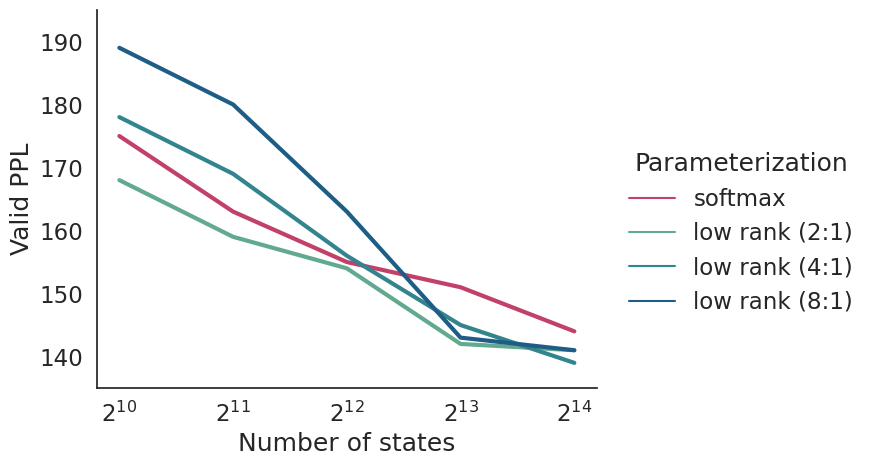
\includegraphics[height=6in]{imgs/hmm/lhmm-states-features-dropout.png}
\caption{HMM Accuracy}
\end{figure}
\begin{figure}
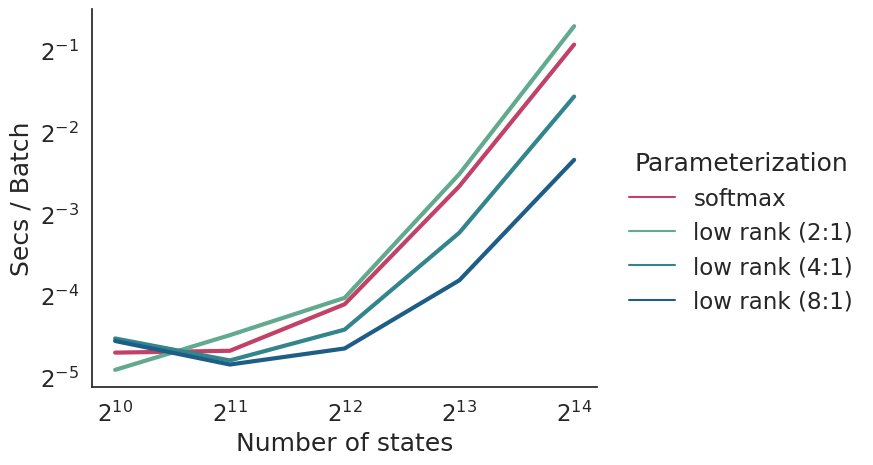
\includegraphics[height=6in]{imgs/hmm/lhmm-states-features-speed-log.png}
\caption{HMM Speed}
\end{figure}
\end{block}

%----------------------------------------------------------------------------------------

\end{column} % End of the second column

\begin{column}{\sepwid}\end{column} % Empty spacer column

\begin{column}{\onecolwid} % The third column

\begin{block}{Speed-Accuracy Frontier}
Low-rank HMMs also dominate softmax HMMs on the speed-accuracy frontier.
\begin{figure}
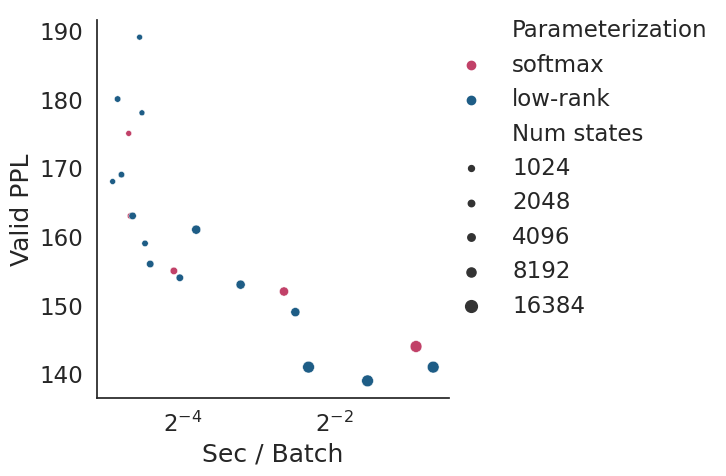
\includegraphics[height=7in]{imgs/hmm/lhmm-speed-accuracy.png}
\caption{Speed-accuracy frontier for HMMs}
\end{figure}
\end{block}

\begin{block}{PCFG Results}
%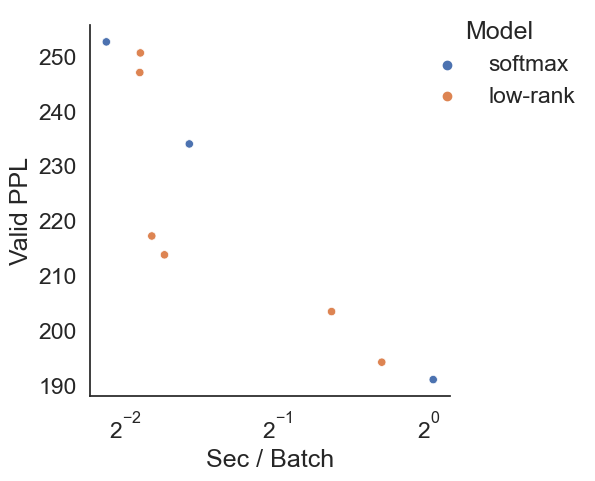
\includegraphics[height=7in]{imgs/hmm/pcfg-speed-accuracy.png}
Low-rank PCFGs (LPCFG) also achieve similar accuracy at faster speeds
(nonterminals $\mcN$, preterminals $\mcP$)
\begin{table}
\centering
\begin{tabular} {lllrrrr}
\toprule
$|\mathcal{N}|$ & $|\mathcal{P}|$ & Model & $R$ &  PPL & Sec/batch\\ %Batch/s\\
\midrule
30  & 60    & PCFG & - & 252.60 &  0.23\\  %4.37\\
    &       & LPCFG & 8 &  247.02    & 0.27\\ %3.75\\
    &       & LPCFG & 16 & 250.59    & 0.27\\ %3.74\\
\midrule
60  & 120   & PCFG & - & 234.01 &  0.33\\ %2.99\\
    &       & LPCFG & 16& 217.24 & 0.28\\ %3.55\\
    &       & LPCFG & 32& 213.81 & 0.30\\ %3.35\\
\midrule
100 & 200   & PCFG & - &  191.08   & 1.02\\ %0.98\\
    &       & LPCFG & 32& 203.47 & 0.64\\ %1.56\\
    &       & LPCFG & 64& 194.25 & 0.81\\ %1.24\\
\bottomrule
\end{tabular}
\end{table}
\end{block}

%----------------------------------------------------------------------------------------
%	CONCLUSION
%----------------------------------------------------------------------------------------

\begin{block}{Conclusion}

Low-rank constraints speed up marginalization
\begin{itemize}
\item Only need to constrain bottleneck parameters
\item Most effective with large models
\end{itemize}

Please see the paper for more experiments:
\begin{itemize}
\item Combination with other structure that admit fast matrix-vector products
\item More datasets (polyphonic music, video) and models (hidden semi-Markov)
\end{itemize}

\end{block}

%----------------------------------------------------------------------------------------
%	REFERENCES
%----------------------------------------------------------------------------------------

%\begin{block}{References}

%\nocite{*} % Insert publications even if they are not cited in the poster
%\small{\bibliographystyle{unsrt}\bibliography{sample}\vspace{0.75in}}
%\printbibliography

%\end{block}

%----------------------------------------------------------------------------------------

\end{column} % End of the third column

\end{columns} % End of all the columns in the poster

\end{frame}


\end{document}
